\documentclass{article}
\usepackage[margin=1in]{geometry}
\usepackage{graphicx}
\usepackage{hyperref}
\usepackage{natbib}
\usepackage{soul}
\usepackage{booktabs}
\usepackage{amsmath}
\bibliographystyle{plain}

\title{Appendix: Quantitative, Multispecies Monitoring at a Continental Scale}

\author{Gledis Guri$^1$\textbf{*} \and
Owen Liu$^2$ \and
Ryan P. Kelly$^1$ \and
Megan R. Shaffer$^1$\and
Kim Parsons$^2$ \and
Ana Ram\'on-Laca$^{1,2,3}$ \and
Krista M. Nichols$^2$ \and
Pedro F. P. Brandão-Dias$^1$ \and
Abigail Wells$^2$ \and
Andrew Olaf Shelton$^2$ \and}

\date{\today}

\begin{document}

\maketitle

\section*{}

\begin{center}
\begin{tabular}{ll}
1 & School of Marine and Environmental Affairs, University of Washington, Seattle, Washington, USA \\
2 & Northwest Fisheries Science Center, NOAA Fisheries, Seattle, Washington, USA \\
3 & Museo Nacional de Ciencias Naturales, Madrid, Spain \\
\hline
\textbf{*} & \textbf{Gledis Guri}, lead and corresponding author \textbf{gguri@uw.edu}
\end{tabular}
\end{center}

\section*{Extended Methods}
\subsection*{qPCR}
Environmental samples were analyzed in triplicate using the multiplexed assay targeting Pacific hake, Eulachon and Pacific lamprey as described in \cite{ramon-laca2021} on a QuanStudio 6 (Applied Biosystems). Only Pacific hake qPCR data was used in this study due to the remaining qPCR targets having little positive amplification. 

The samples underwent real-time thermocycler protocol including an initial denaturation step at 95°C 10 min followed by 45 cycles of 15 s at 95°C and 1 min at 60°C. All samples were run in 10 $\mu$L volume consisting of 1 x TaqPath ProAmp Multiplex Master Mix, 0.9 $\mu$M of each primer (forward: AAATGTTTAAACTAGAGCCGAATAGC and reverse: TCGTGGAGTCAAAGTGGGGTAGA), 0.2 $\mu$M of probe (6FAM-CACTCGAGGCCACGAAGTACAATT-(MGB)NFQ), and 2 $\mu$L of DNA template or water for the non-template control. All reactions included 100 copies of internal positive control (IPC) to detect PCR inhibition. Any IPC delay exceeding 0.5 cycles in the non-template control was considered inhibition and inhibited samples were diluted and re-analyzed. 

Alongside environmental samples standard samples were analyzed constructed from a 130 bp synthetic DNA fragment (gBlock; IDT) representing the 12S region of Pacific hake (\textit{Merluccius productus}), which encompasses the 101 bp 12S qPCR target (sequence information available in \cite{ramon-laca2021}). The synthetic DNA fragment was diluted to create a series of standards with final concentrations ranging from $10^{0}$ to $10^{5}$ copies/$\mu$L.

\subsection*{Metabarcoding}
In total, 568 samples, including 554 environmental samples, 7 PCR blanks and 7 positive controls (holding only kangaroo DNA) were amplified using MiFish-U universal primers \cite{miya2015} with Illumina tails (forward TCGTCGGCAGCGTCAGATGTGTATAAGAGACAGGCCGGTAAAACTCGTGCCAGC; reverse GTCT- CGTGGGCTCGGAGATGTGTATAAGAGACAGCATAGTGGGGTATCTAATCCCAGTTTG) by using a two-step PCR protocol. The DNA was amplified in the first PCR reaction (PCR1) in a 20 µL reaction consisting of: 10 µL of Phusion Master Mix (2X), 0.4 µL of the forward primer (10 µM); 0.4 µL of the reverse primer (10 µM), 0.6 µL of 100\% DMSO, 0.5 µL of rAlbumin (20 µg/µL), 4.4 µL of nuclease-free water and 2 µL of DNA template. Reactions were run with the following cycling conditions: an initial denaturation of 98°C for 30 sec; followed by 35 cycles of 98°C for 10 sec, 60°C for 30 sec, and of 72°C for 3 sec; with a final extension of 72°C for 10 min and hold at 4°C. 

PCR product was cleaned using Ampure Beads (1.2x) and then indexed in a second PCR reaction (PCR2), with the following recipe: 12.5 $\mu$L of KAPA HiFi HotStart ReadyMix (Roche Diagnostics), 1.25 $\mu$L of an index from IDT for Illumina DNA/RNA UD Indexes (Sets A-D), 5 $\mu$L of PCR1 product, and 6.25 $\mu$L of nuclease free water. Cycling conditions included an initial denaturation of 95°C for 5 min; 8 cycles of: 98°C for 20 sec, 56°C for 30 sec, 72°C for 1 min; and a final extension of 72°C for 5 min. Resulting products were visualized on a 2\% agarose gel and quantified using Quant-iT™ dsDNA Assay Kit (Thermo Fisher Scientific, USA) with Fluoroskan™ Microplate Fluorometer (Thermo Fisher Scientific, USA). Indexed products were normalized by concentration, pooled into libraries for sequencing, and then size- selected to extract only the target fish band using the E-Gel™ SizeSelect™ II Agarose Gels (Thermo Fisher Scientific, USA).  Subsequently the libraries were sequenced on Illumina MiSeq platform using the v3 600 cycle kit. 


\subsection*{Mock community}

We constructed mock communities with even and skewed species total genomic DNA using Qubit HS assay quantification method. We then quantified the concentration of the 12S rRNA gene using MarVer1 primers (forward: CGTGCCAGCCACCGCG; reverse: GGGTATCTAATCCYAGTTTG \cite{valsecchi2020}), which perfectly matched the template to give unbiased estimates of concentration, using ddPCR (Bio-Rad, Inc., QX200 Droplet Digital PCR system). Each tissue of each species was quantified in a 22 $\mu$L reaction consisted of 2 $\mu$L of DNA template from genomic DNA , 11 $\mu$L of ddPCR EvaGreen (Bio-Rad), 0.22 $\mu$L of each forward and reverse primers (10 uM), and 0.56 $\mu$L of nuclease free water. The thermocycler reactions were run in C1000 Touch Thermal Cycler with 96-Deep Well Reaction Module (Bio-Rad) using the PCR program as follows: 2 min at 50°C for enzyme activation, 2 min at 95°C for initial denaturation, and 40 cycles of denaturation for 1 sec at 95°C and primer annealing and elongation for 30 sec min at 60°C, with a ramp rate of 2°C per s and heldat 4°C until droplets were read. Droplets were determined to be positive after drawing a threshold based on NTCs.

\subsection*{Bioinformatics}
Starting with Illumina-demultiplexed sequencing files, we first removed primer and adapter sequences using Cutadapt v4.9, applying the default mismatch tolerance parameter (-e 0.1) \cite{martin2011}. Next, we performed quality filtering using the filterAndTrim function from the dada2 R package, retaining its default parameters while specifying the optional truncLen argument to match the minimum MiFish amplicon length. After filtering, we denoised the sequences using dada2 with default settings \cite{callahan2016}, which resulted in a list of Amplicon Sequence Variants (ASVs) across all samples. Each resulting ASV was then assigned a unique 28-character hash code using the sha-1 algorithm with the R function map\_chr. This allowed us to create a common database of ASVs by hash, enabling us to track which sequences have already been annotated for consistency and to avoid redundant computational efforts.

For taxonomic assignment of ASVs, we used standalone BLAST \cite{altschul1990} to compare each unique ASV against the NCBI nr eukaryote database as of January 2025. BLAST arguments were as follows: "-word\_size 30 -evalue "1e-30" -max\_target\_seqs 50". To streamline annotation, we also used the "-negative\_taxids" argument, including a list of target organisms closely related to those present in the sampled region, but known to be absent. The complete list of taxids that were excluded is available alongside the pipeline code. Finally, we performed a least common ancestor (LCA) analysis on the top BLAST hits using TaxonKit v0.17 \cite{shen2021}. Sequences with a 100 percent identity match to any database sequence were prioritized for LCA. In the absence of perfect matches, we conducted LCA analysis on the top hits with identity scores above 99.3, , 98, or 96 percent respectively. In the absence of any hits above 96 identity, taxonomic assignment was truncated. Finally, for mock communities were identify of species was known, we manually curated annotations before analysis. 

\subsection*{Statistical model}

\subsubsection*{Overview}

We developed a joint model for modeling DNA concentration in the coastal ocean using single-species qPCR data Pacific hake and metabarcoding data from the 12S MiFish Universal primer. This work builds off previous single-species eDNA models constructed for Pacific hake (Shelton et al. 2022) and models for joining qPCR and metabarcoding data (Guri et al. 2024). Here qPCR observations provide information about DNA concentration for one species (Pacific hake) and the metabarcoding data provide information about species composition within a sample (i.e. proportions that sum to one).  In combination, these two data sources allow for estimation of DNA concentrations for all species observed by metabarcoding.

\subsubsection*{qPCR model}

We developed a state-space framework for modeling hake DNA concentration in the coastal ocean building and modifying the work of Shelton et al. (2022).  State-space models separate the true biological process from the methods used to observe the process. Let $D_H(x,y,d)$ be the true, but unobserved concentration of hake DNA (log DNA $copies$ $\mu L^{-1}$) present at spatial coordinates $\{x,y\}$ (eastings and northings, respectively, in km) and sample depth $d$ (meters). Hereafter we refer to a combination of spatial location and depth as a ``station". Let $\psi_0$ be the intercept representing the mean hake DNA concentration and $\epsilon(x,y,d)$ be a random effect that allows for the effect of spatial location and water depth. We write these as additive on the log-scale,

\begin{align}
  D_H(x,y,d) &= \psi_0 + \epsilon(x,y,d) \\
  \epsilon(x,y,d) &\sim N(0,\sigma_D)
\end{align}

This model describes perhaps the simplest possible random effect model and notably does not leverage any information about the spatial arrangement of samples (i.e. the random effect does not include a spatial correlation component).  This is intentional.  The focus of this model is on the other species DNA concentration (not Pacific hake) and therefore we allow the estimated hake concentrations at a to follow the qPCR observations as much as possible. 

Unfortunately, qPCR does not directly measure DNA concentration. Instead qPCR measures the PCR cycle at which a 2$\mu L$ aliquot of a extacted DNA was detected to fluoresce and compares that observation against the flourescence pattern of samples of known DNA concentration ("the standard curve"). This provides an estimate of DNA concentration for each unknown sample. Each water sample is analyzed using at least 3 independent qPCR replicates to account for laboratory and machine variability. In addition to qPCR variability among replicates, we also have to account for modifications that affect each water sample and occurred during water sampling and processing. First, we have three offsets that modify the true DNA concentration to affect what we observed in the qPCR. For water sample $i$: 1) $V_i$ is the proportion of 2.5 L filtered from Niskin $i$ (occasionally some seawater was spilled or not filtered; $V_i =1$ for the vast majority of samples); 2) $I_i$ is the known dilution used to on sample $i$ to eliminate PCR inhibition. PCR inhibition is most commonly observed in surface samples and is vanishingly rare for samples collected below 100m; 3) $\mathbf{I}\zeta$ is an estimated offset for an ethanol wash error ($\zeta$ is the estimated effect of the wash error and $\mathbf{I}$ is an indicator variable where $\mathbf{I}=1$ for affected samples and $\mathbf{I}=0$ otherwise; see Shelton et al. 2022 Supp S1 for additional description). Here we fix $\zeta$ = XXX based on previous analyses (Shelton et al. 2022).

Finally, we add a random effect for the individual bottles sampled at each year-station-depth combination ($\delta_i(x,y,d)$). This effect  describes the deviation of individual sampled bottles from the location mean, $\delta_i(x,y,d) \sim N(0,\sigma_D)$, with $\sigma_D$ indicating a depth-specific standard deviation among bottles. Because we have only two replicate bottles at each location, we impose a sum to zero constraint on the bottles collected from a single location (i.e. for a given location, $\sum_i \delta_i(x,y,d) = 0$). Then, the log-concentration of hake DNA in a sample analyzed by qPCR, $E_{Hi}$ is, 

\begin{align}
  E_{Hi} &= D_H({x,y,d}) +  \log{V_i} + \log{I_i} + \mathbf{I}\zeta + \delta_i(x,y,d)
\end{align}

We connect the estimated concentrations to observations from qPCR using two likelihoods connected to the concentration $E$. First we determine whether amplification was detected in each qPCR replicate $r$ run on each plate $j$, $Z_{Hijr}$ and if amplification was observed we model the PCR cycle at which amplification was detected $Y_{Hijr}$; $Y_{Hijr}$ is observed as a continuous, positive value. DNA concentrations have a log-linear relationships with $Y_{Hijr}$; smaller values of $Y_{Hijr}$ are associated with higher DNA concentrations. 

Because we are modeling the discrete number of DNA molecules that are present in the assayed sample, we know that the Poisson distribution provides an appropriate observation distribution for the number of molecules present in a given qPCR reaction. Assuming a Poisson distribution, conditional on a true mean number of DNA copies in the sample $X$, the probability of having exactly zero DNA copies in a qPCR reaction is $e^{-X}$ and the probability of having non-zero DNA copies is the complement, $1-e^{-X}$. If there are exactly zero molecules in a qPCR reaction, amplification and therefore detection of amplification will not occur. However, there are other factors (e.g. PCR inhibition) that may reduce amplification further and therefore we expect the probability of amplification to be at most $1-e^{-X}$. As a result, we estimate an additional term, $\phi$ representing the fractional reduction in amplification efficiency due to other factors on qPCR plate $j$ ($0<\phi<1$). Then we have a pair of observation models for hake DNA, both of which are a function of DNA concentration, $E_{Hi}$

\begin{align}
  Z_{Hijr} &\sim Bernoulli\left(1 - \exp(-2 e^{E_{Hij}}\phi) \right) \\ 
  Y_{Hijr} &\sim Normal \left(\beta_{0j}+\beta_{1j}{E_{Hij}},\sigma_Y(E_{Hij}) \right) \qquad  if \: Z_{Hijr} = 1 
\end{align} 

The 2 is present in the first line of the equation because we use 2 $\mu L$ of sample in each qPCR reaction and so the expected DNA copies in reaction is $2e^{E_{ij}}$. We allow $\sigma_C(E_{ij})$ to vary as a log-linear function of DNA concentration to account for the fact that there is decreased variability in qPCR measures of $C_t$ at higher DNA concentrations: $\sigma_C({E_{ij}}) = exp(\gamma_{0}+\gamma_{1}E_{ij})$.

By itself, the above model is unidentifiable because field samples do not provide information about the parameters that define relationship between the number of DNA copies and PCR cycle ($\beta_{0j}$, $\beta_{1j}$, and $\phi$). As is standard with qPCR analyses, we include standards of known concentration to estimate these parameters. Each qPCR plate has replicate samples with a known number of DNA copies. These standards span six orders of magnitude (1 to 100,000 copies $\mu L^{-1}$, each of 2$\mu L$) and determine the relationship between copy number and PCR cycle of detection. Let $K_{jp}$ be the known log-copy number for sample $j$ in PCR plate $p$, then,

\begin{align}
  Z_{jp} &\sim Bernoulli \left(1-exp(-2 e^{K_{jp}} \phi) \right)\\
  Y_{jp} &\sim Normal \left(\beta_{0j}+\beta_{1j}{K_{jp}},\sigma_Y(K_{jp})\right) \quad  if \: Z_{jp} =1
\end{align}

Note that there are different intercept ($\beta_{0p}$) and slope ($\beta_{1p}$) parameters for each PCR plate to allow for among-plate variation in amplification. We model each calibration parameter ($\beta_{0p},\beta_{1p})$ hierarchically using a normal distribution, with among plate mean and variance (i.e. $\beta_{0p} \sim N(\mu_{\beta_{0}},\sigma_{\beta_{0}})$).

\subsubsection*{Metabarcoding model}

In addition to the qPCR observations, we used the MiFish primer and high throughput sequencing to detect and enumerate the sequences of other fish species in the same samples that were examined for hake DNA. Again, we are interested in determining the DNA concentration of each focal species in each sample. Unfortunately, metabarcoding data is compositional data \cite{glor2017, shelton2023}, and so while it can inform the relative abundance of species within a sample, alone it cannot provide estimates of DNA concentration. Fortunately, the qPCR data from Pacific hake provides information about DNA concentration for one species and the metabarcoding data provides information about the relative abundance for tens of species, including hake. Here, we follow and extend the metabarcoding model developed by Shelton et al. (2023) and show how it links with the qPCR model above. 

As above, we let $D_s(x,y,d)$ be the log-scale eDNA concentration but now for species $s$. We let $E_{si}(x,y,d)$ be the log-DNA concentration for each species in each bottle. Importantly one of the $s$ species is Pacific hake and so connects to the qPCR model above. Metabarcoding reads are compositional and so we model the DNA concentration relative to one another using the additive log-ratio transformation (ALR; \textbf{Aitchison 1986}).  We define a reference species in each sample, $R$, with the species used as a reference varying among sample. Let $\alpha_s$ be the per PCR cycle log amplification rate for species $s$ (see \cite{shelton2023}).  We can then calculate $\nu_{si}$, the log-ratio between species $s$ and the reference species after accounting for amplification bias (see *Mock Communities* below),

\begin{align} 
  \nu_{si} &= \left( E_{si}(x,y,d) - E_{Ri}(x,y,d)\right) + N_{PCR} \left(\alpha_s - \alpha_{Ri} \right) 
\end{align}

We can then convert the $\nu$s to the predicted proportions of the metabarcoding reads $\mu_{si}$ using the softmax transformation and to the observed reads via a Multinomial likelihood,

\begin{align} 
  \pi_{si} &= \dfrac{e^{\nu_{si}}}{\sum_{s=1}^S e^{\nu_{si}}} \\
  \boldsymbol{R}_{i} & \sim Multinomial\left(\boldsymbol{\pi}_{i},T_{i}\right) 
\end{align}

where $T_{i}$ is the total number of reads observed across all species for that bottle. 

As with the qPCR analyses, in the absence of additional information estimates of $\alpha$ and $E$ cannot be statistically identified.  We use the mock community data, which has known input DNA concentrations and  same basic model as for the metabarcoding observations but instead of having unknown DNA concentrations, we have known inputs for each species $L_{sm}$ in mock community $m$. Then:

\begin{align} 
 \nu_{sm} &= \left( L_{sm} - L_{Rm}\right) + N_{PCR} \left(\alpha_s - \alpha_{Ri} \right) \\
  \pi_{sm} &= \dfrac{e^{\nu_{sm}}}{\sum_{s=1}^S e^{\nu_{sm}}} \\
  \boldsymbol{R}_{m} & \sim Multinomial\left(\boldsymbol{\pi}_{m},T_{m}\right) 
\end{align}

To maintain identifiability, we assign one $\alpha_s = 0$. (ADD. WHICH ONE IS ZERO?, WHICH IS THE REF SPECIES?). ADD PLOT of ALPHAS.



\subsubsection*{Smoothing predictions}

Ole's questions:
Smoothed model is based on E (a single water bottle), not D.
What was used in the making the smooth?  Posterior mean?

\textbf{OWEN.  COULD YOU HELP HERE?}

The above statistical model provides predictions of species-specific DNA concentrations ($E$) at each depth sampled (d = 0, 50, 150, 300 or 500 m). We used the sdmTMB package \cite{anderson2022} to generate distribution models for the concentration of eDNA , as:
$$E_i(xyz) = \tau + \eta(s) + \varepsilon_{d}(s)$$
where x,y,z index longitude, latitude, and depth, respectively, $\tau$ is scalar intercept, $\eta(s)$ is a spatial smooth shared among depths, and $\varepsilon_d(s)$ is a depth-specific spatial smooth. Both $\eta(s)$ and $\varepsilon_d(s)$ are a zero-centered Gaussian random field estimated using the stochastic partial differntial equation (SPDE) approximation (see \cite{anderson2022}). Each species was fitted individually while we created and selected the best mesh for approximating spatial Gaussian random fields as part of the model.

\subsection*{Model convergance}

Gelman-Rubin statistics.  Predicted-observed, etc.


%%% Each figure should be on its own page
\begin{figure}
\centering
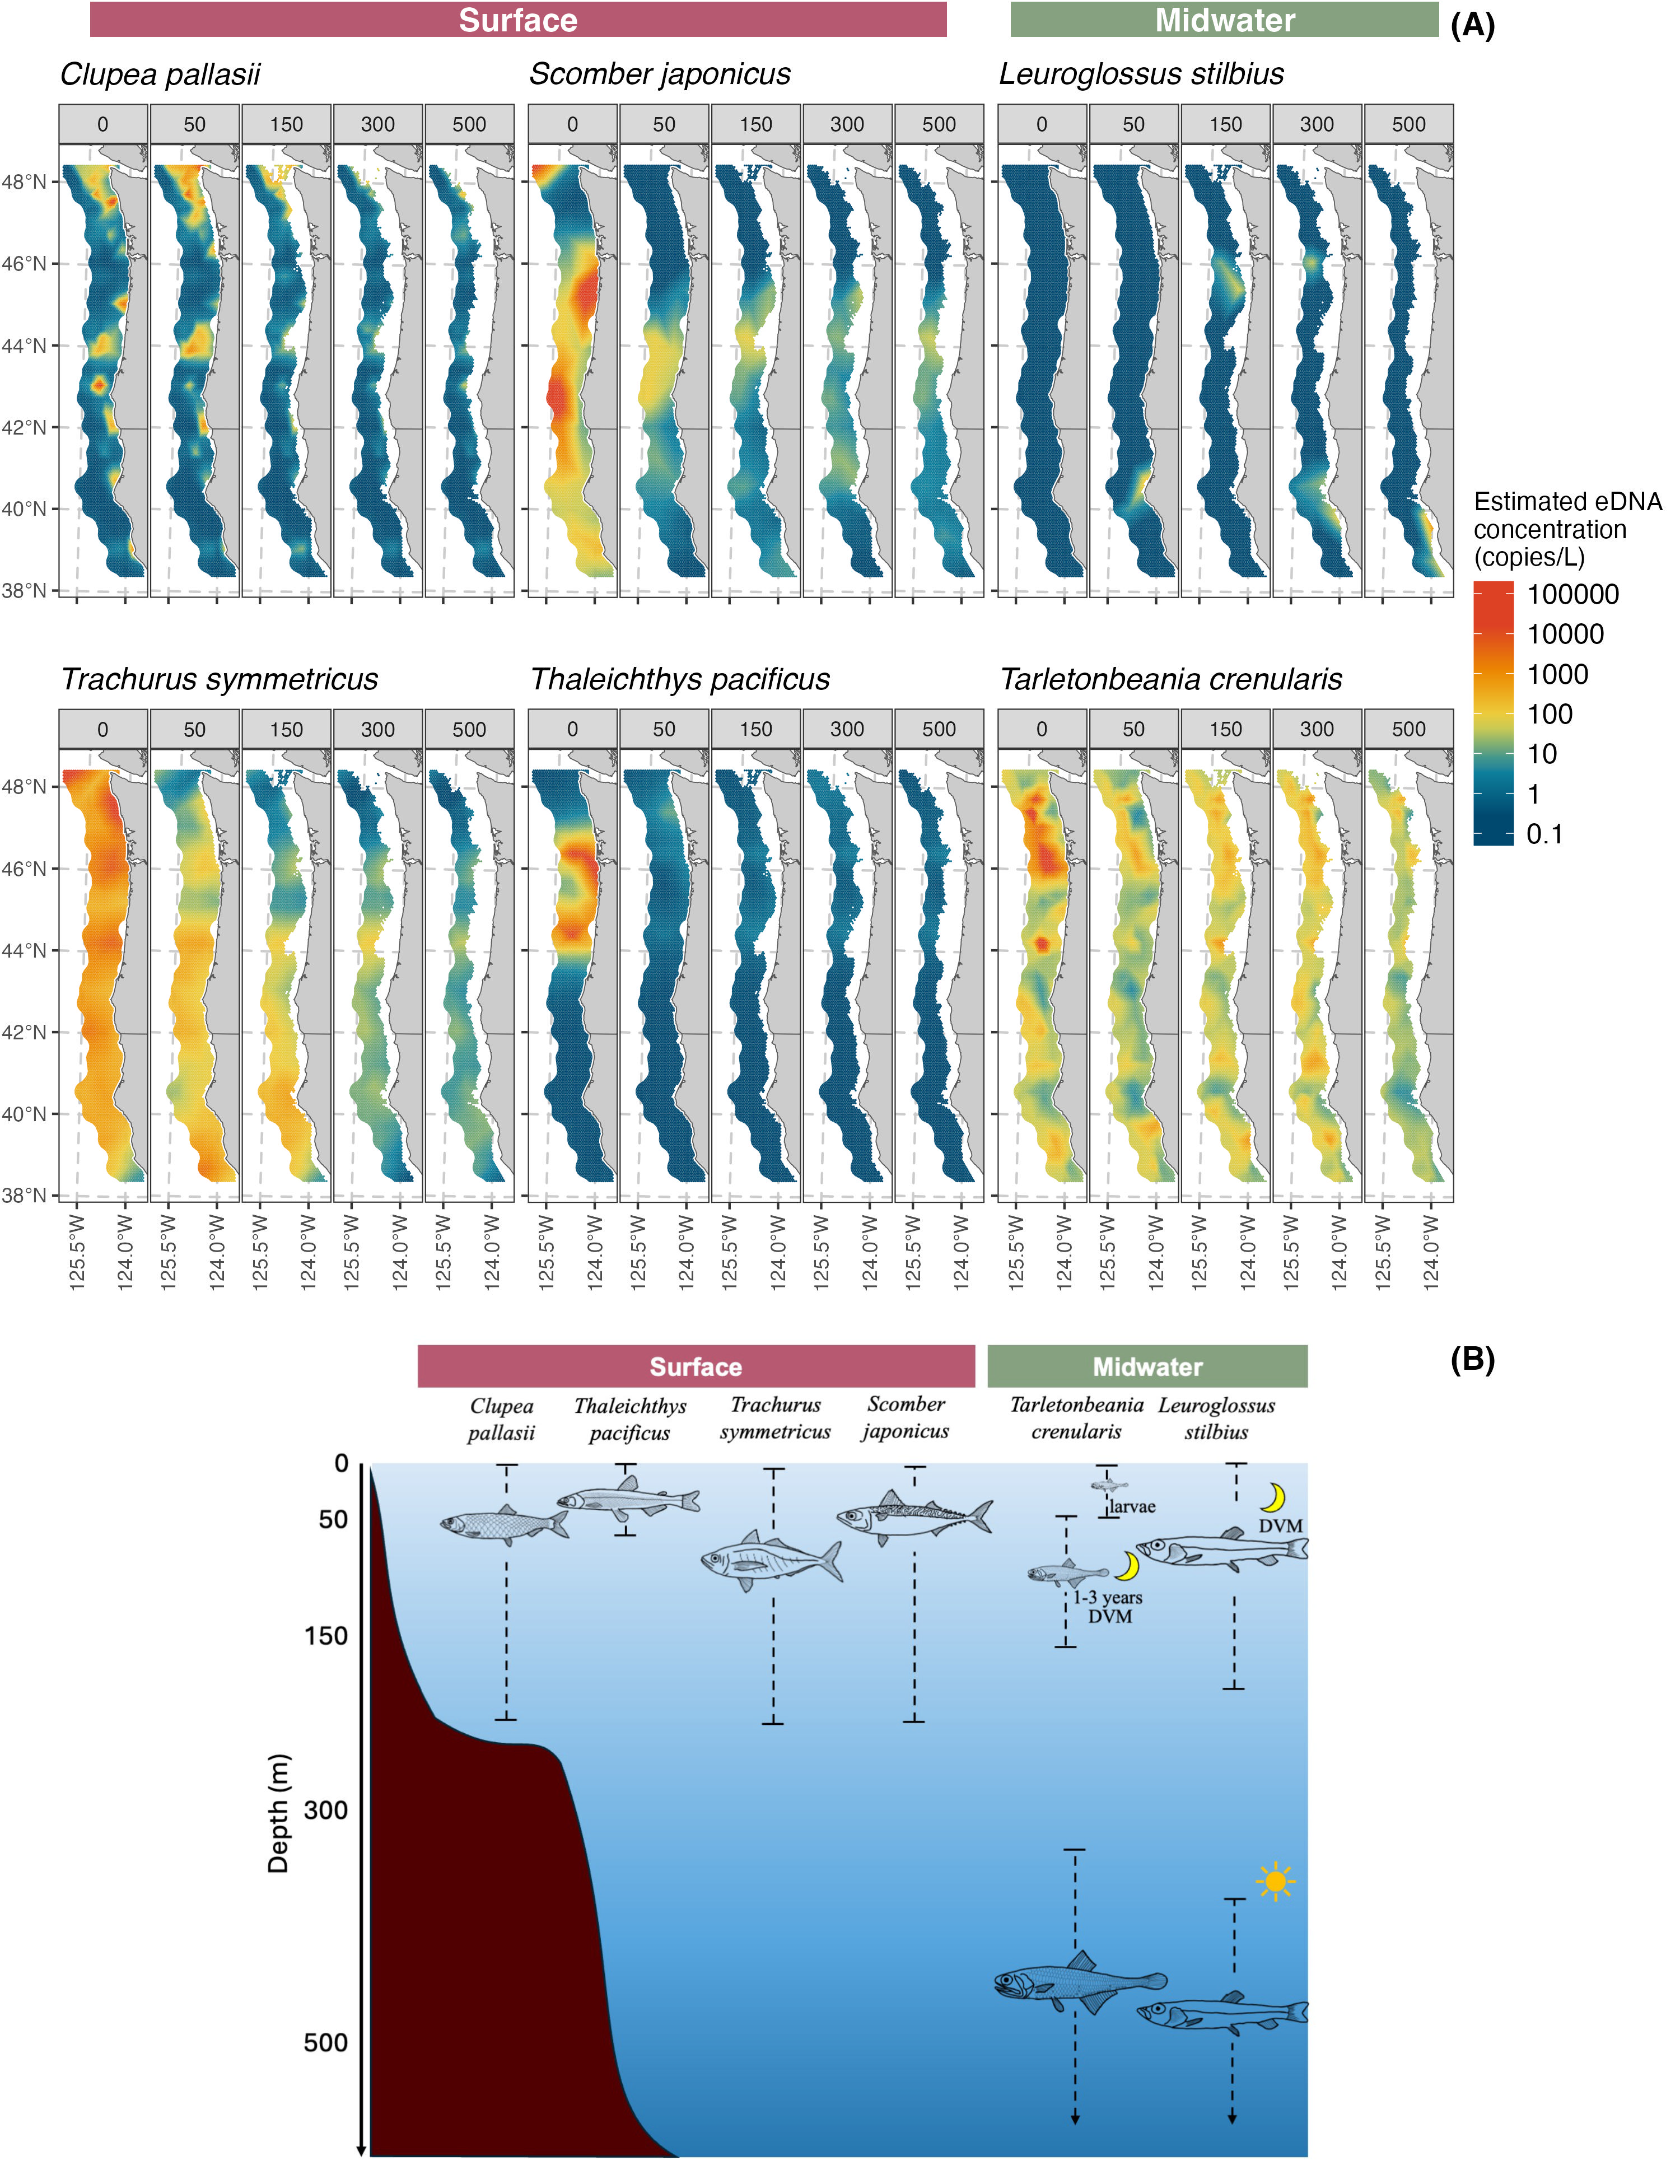
\includegraphics[width=0.90\textwidth]{plots/5_Supplementary_Figure_1.jpg}
\caption{Continuation of Fig. 1. Estimated species eDNA for \textit{Clupea pallasi}, \textit{Trachurus symmetricus}, \textit{Scomber japonicus}, \textit{Thaleichthys pacificus}, \textit{Leuroglossus stilbius}, and \textit{Tarletonbaeania crenularis} concentration (A) across 0, 50, 150, 300, and 500m depth samples and known depth distribution of those species from literature (B).}
\end{figure}

%%% Each figure should be on its own page
\begin{figure}
\centering
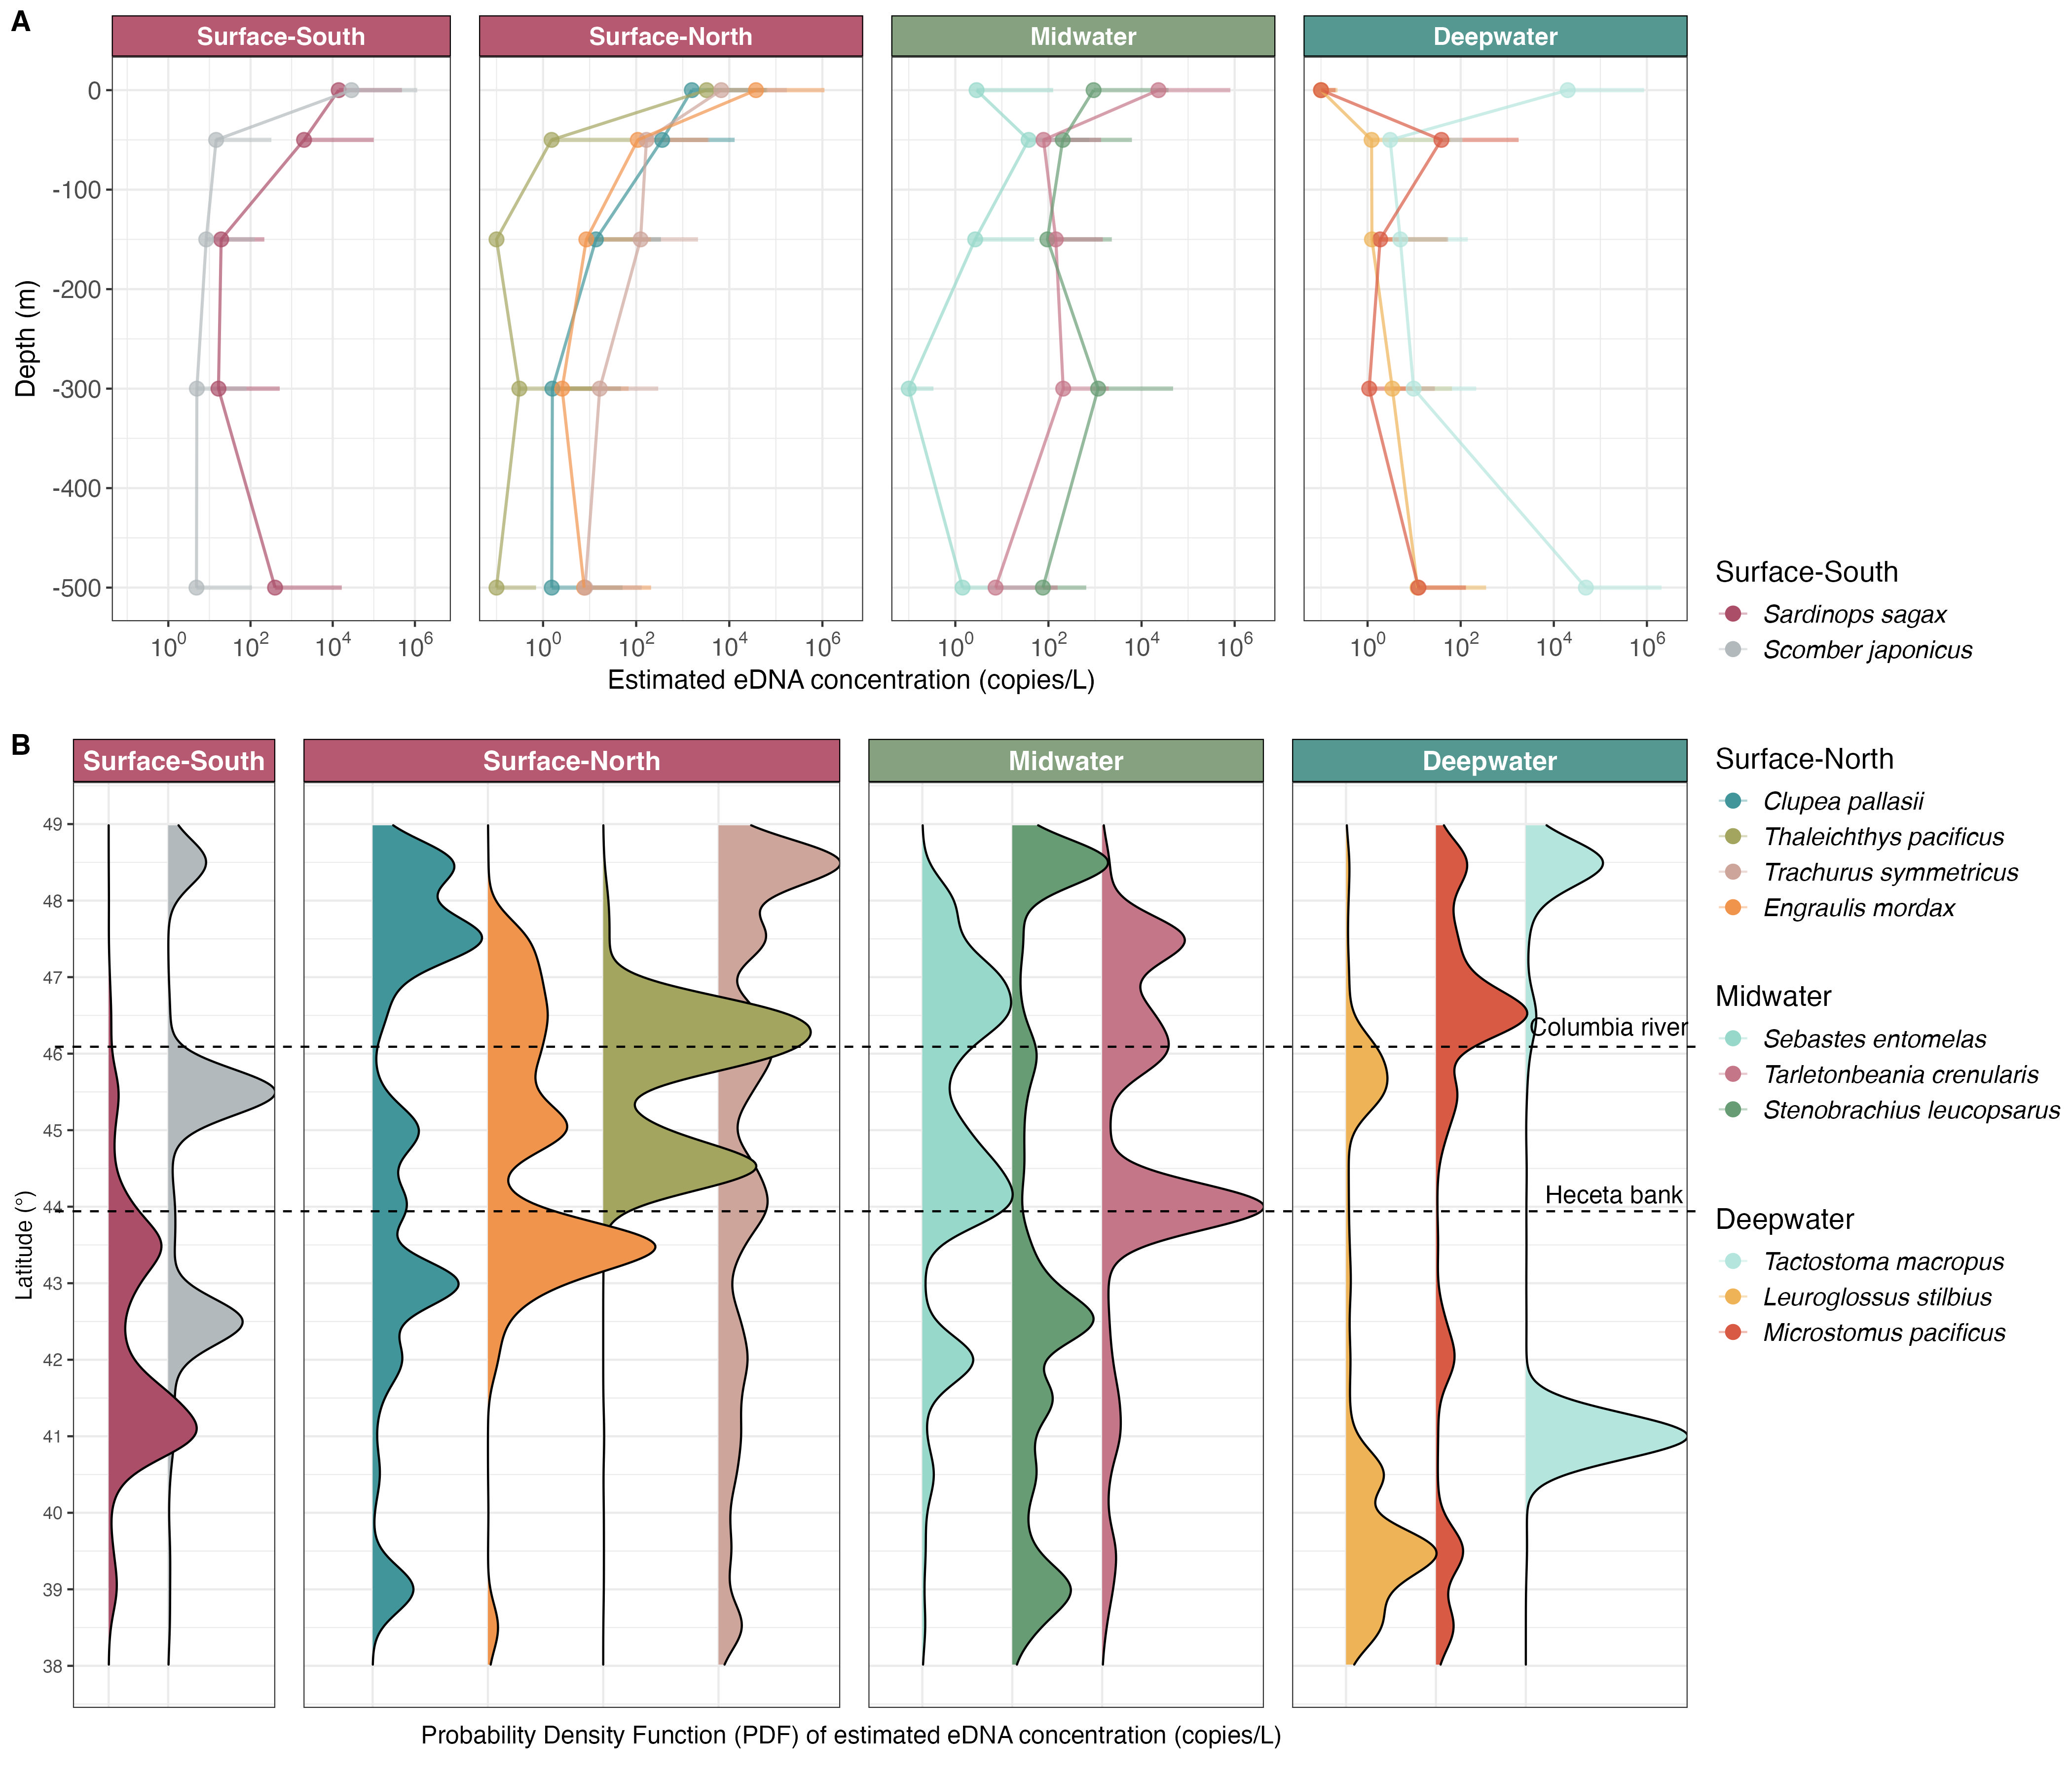
\includegraphics[width=0.89\textwidth]{plots/4_Figure_4.jpg}
\caption{Vertical (A) and latitudinal (B) distribution of eDNA concentrations grouped in ecological groups (surface south, surface north, midwater, and deepwater). Mean eDNA concentration of vertical distribution is shown with dots and 99\% upper quantile with ticks (A). Probability density functions (PDF) of estimated eDNA concentrations across latitudinal gradients (B; square root transformed of x-axis to enhance low concentration peaks). Key geographic features, such as the Columbia River and Heceta Bank, are marked to indicate alignment of species distributions.}
\end{figure}

%%% Each figure should be on its own page
\begin{figure}
\centering
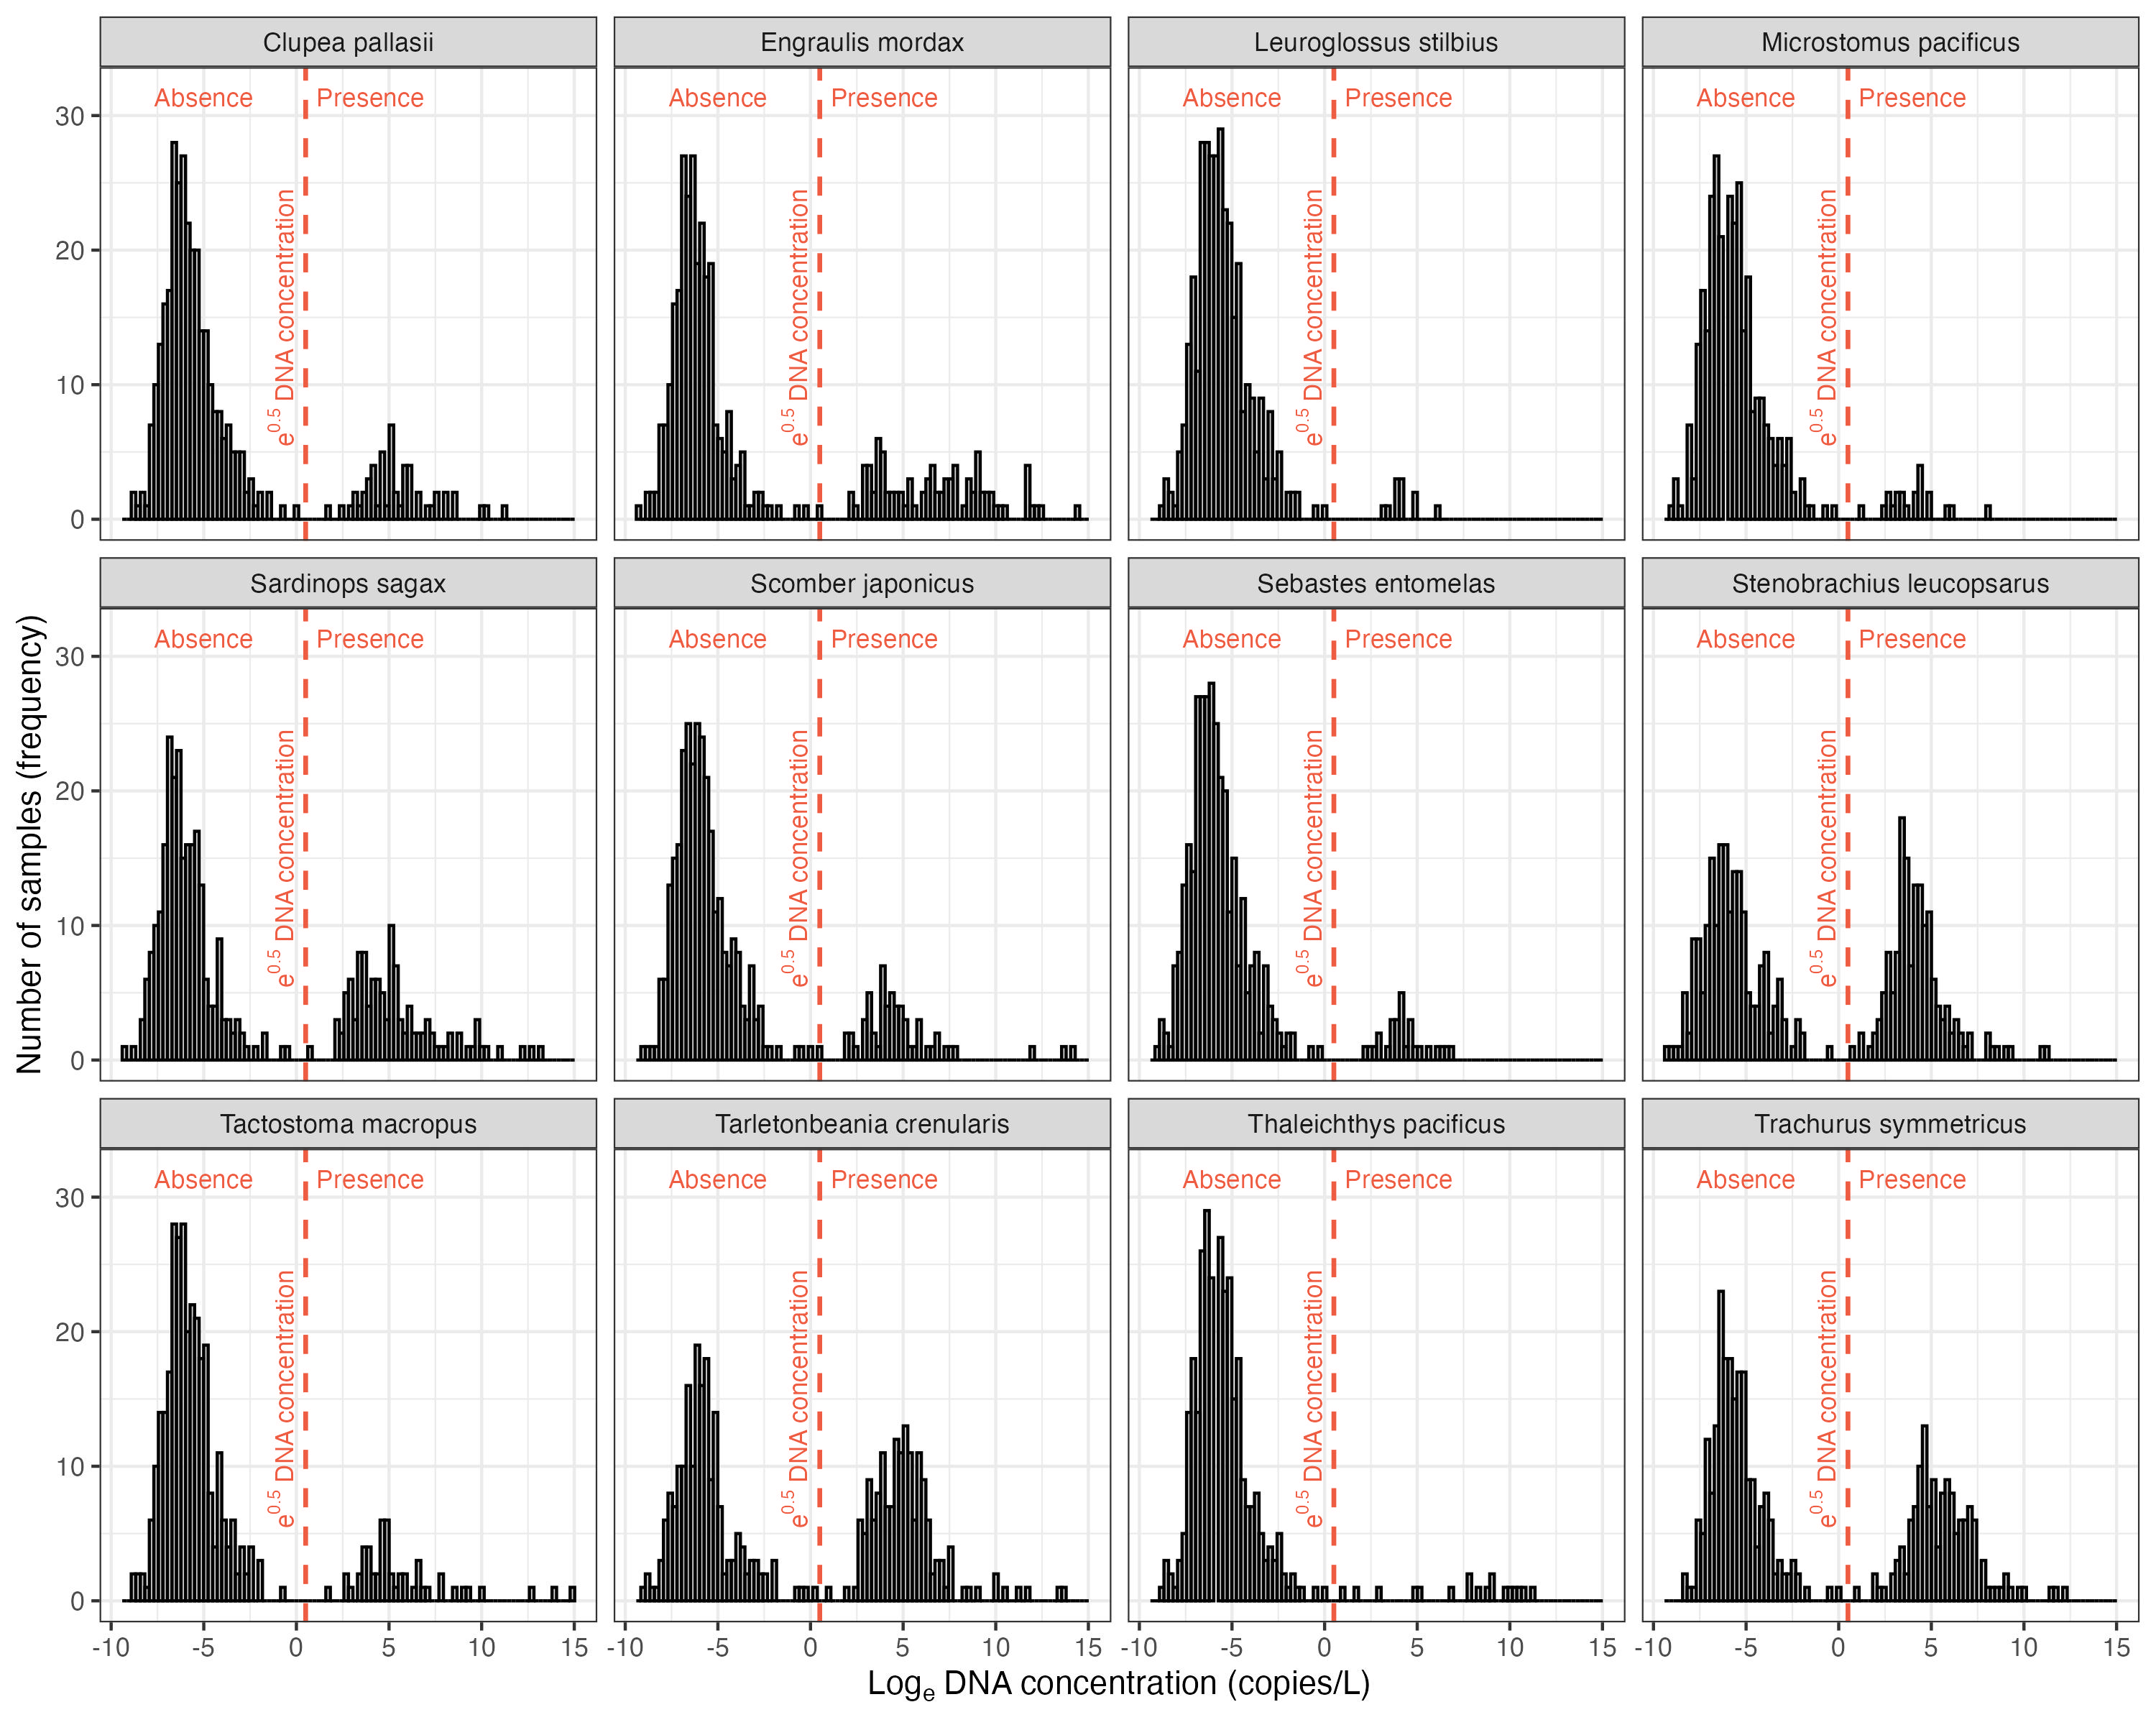
\includegraphics[width=0.99\textwidth]{plots/6_Supplementary_Figure_2.jpg}
\caption{Frequency distribution of eDNA concentration for each species included in this study (n = 12). The dashed red line indicates the threshold model estimated concentration (copies/L) for defining presence and absence of sequenced (through metabarcoding) taxa}
\end{figure}

%%% Each figure should be on its own page
\begin{figure}
\centering
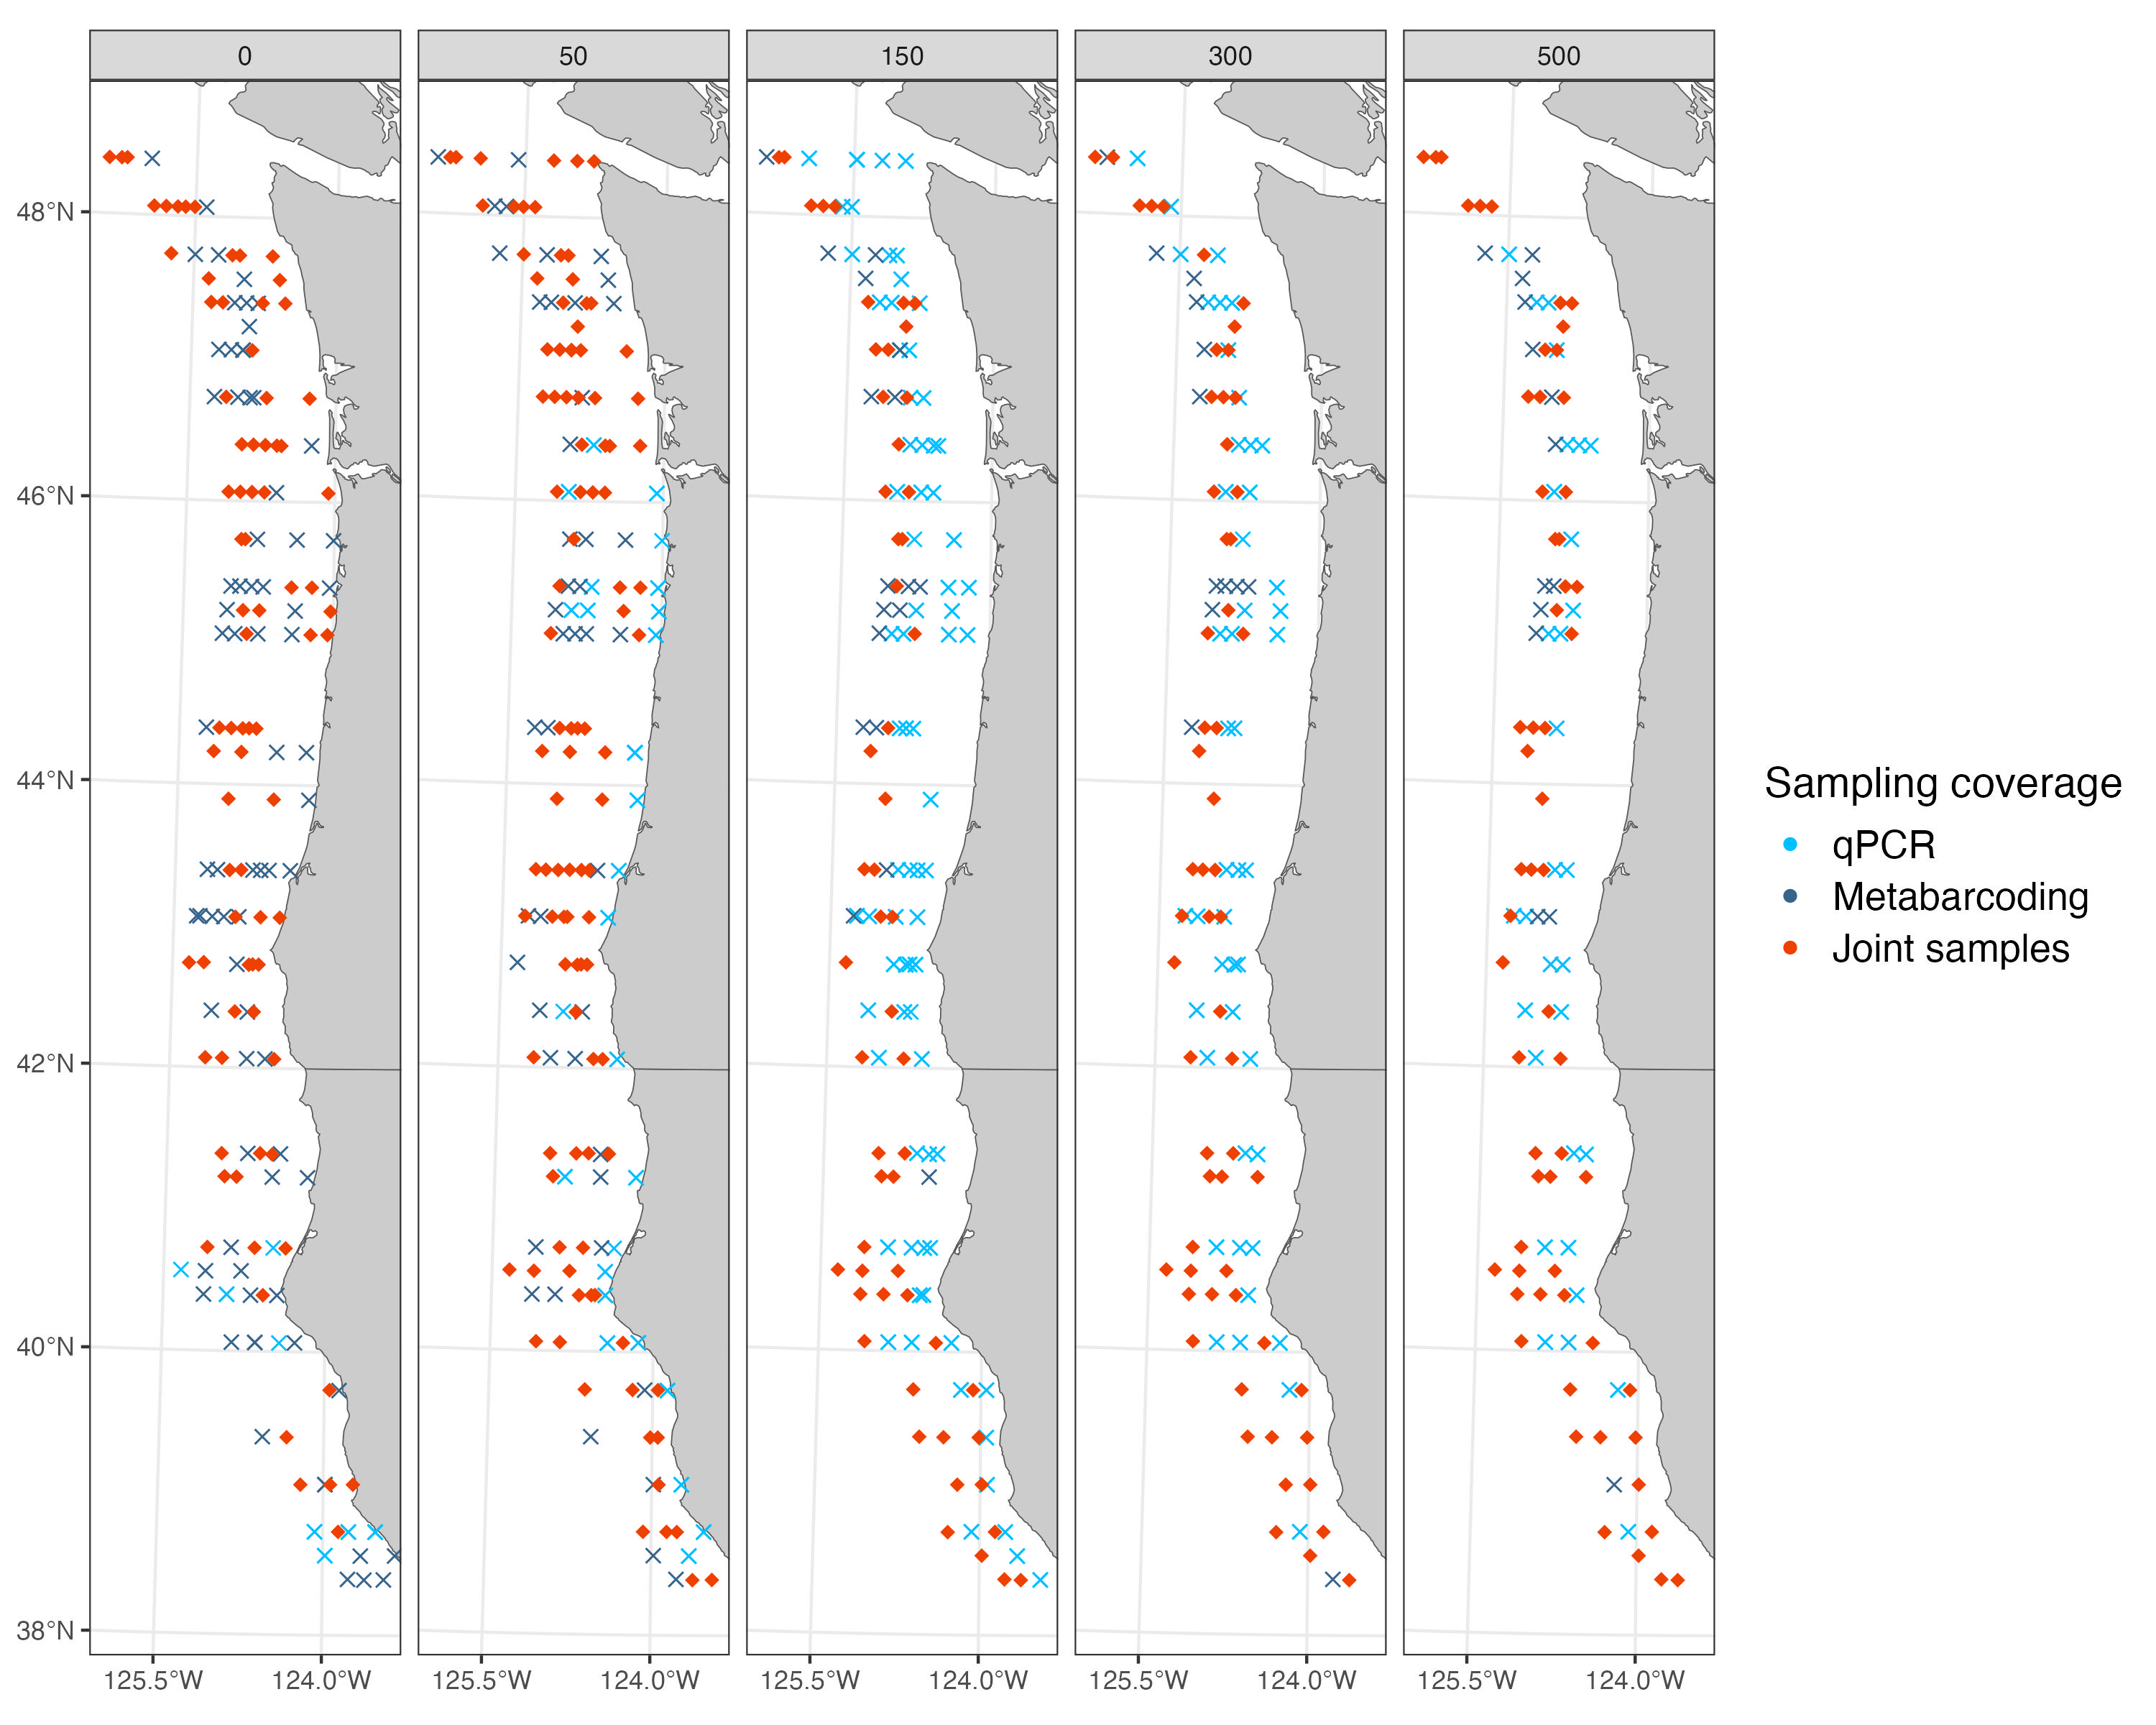
\includegraphics[width=0.99\textwidth]{plots/7_Supplementary_Figure_3.jpg}
\caption{Three-dimensional distribution of samples collected that were run through qPCR (light blue), metabarcoding (dark blue), and were used jointly in the Bayesian model (Fig. 4; red). Jointly modeled samples are those that detected Pacific hake -- used as a reference species for quantification -- in both qPCR and metabarcoding assays.}
\end{figure}

%%% Each figure should be on its own page
\begin{figure}
\centering
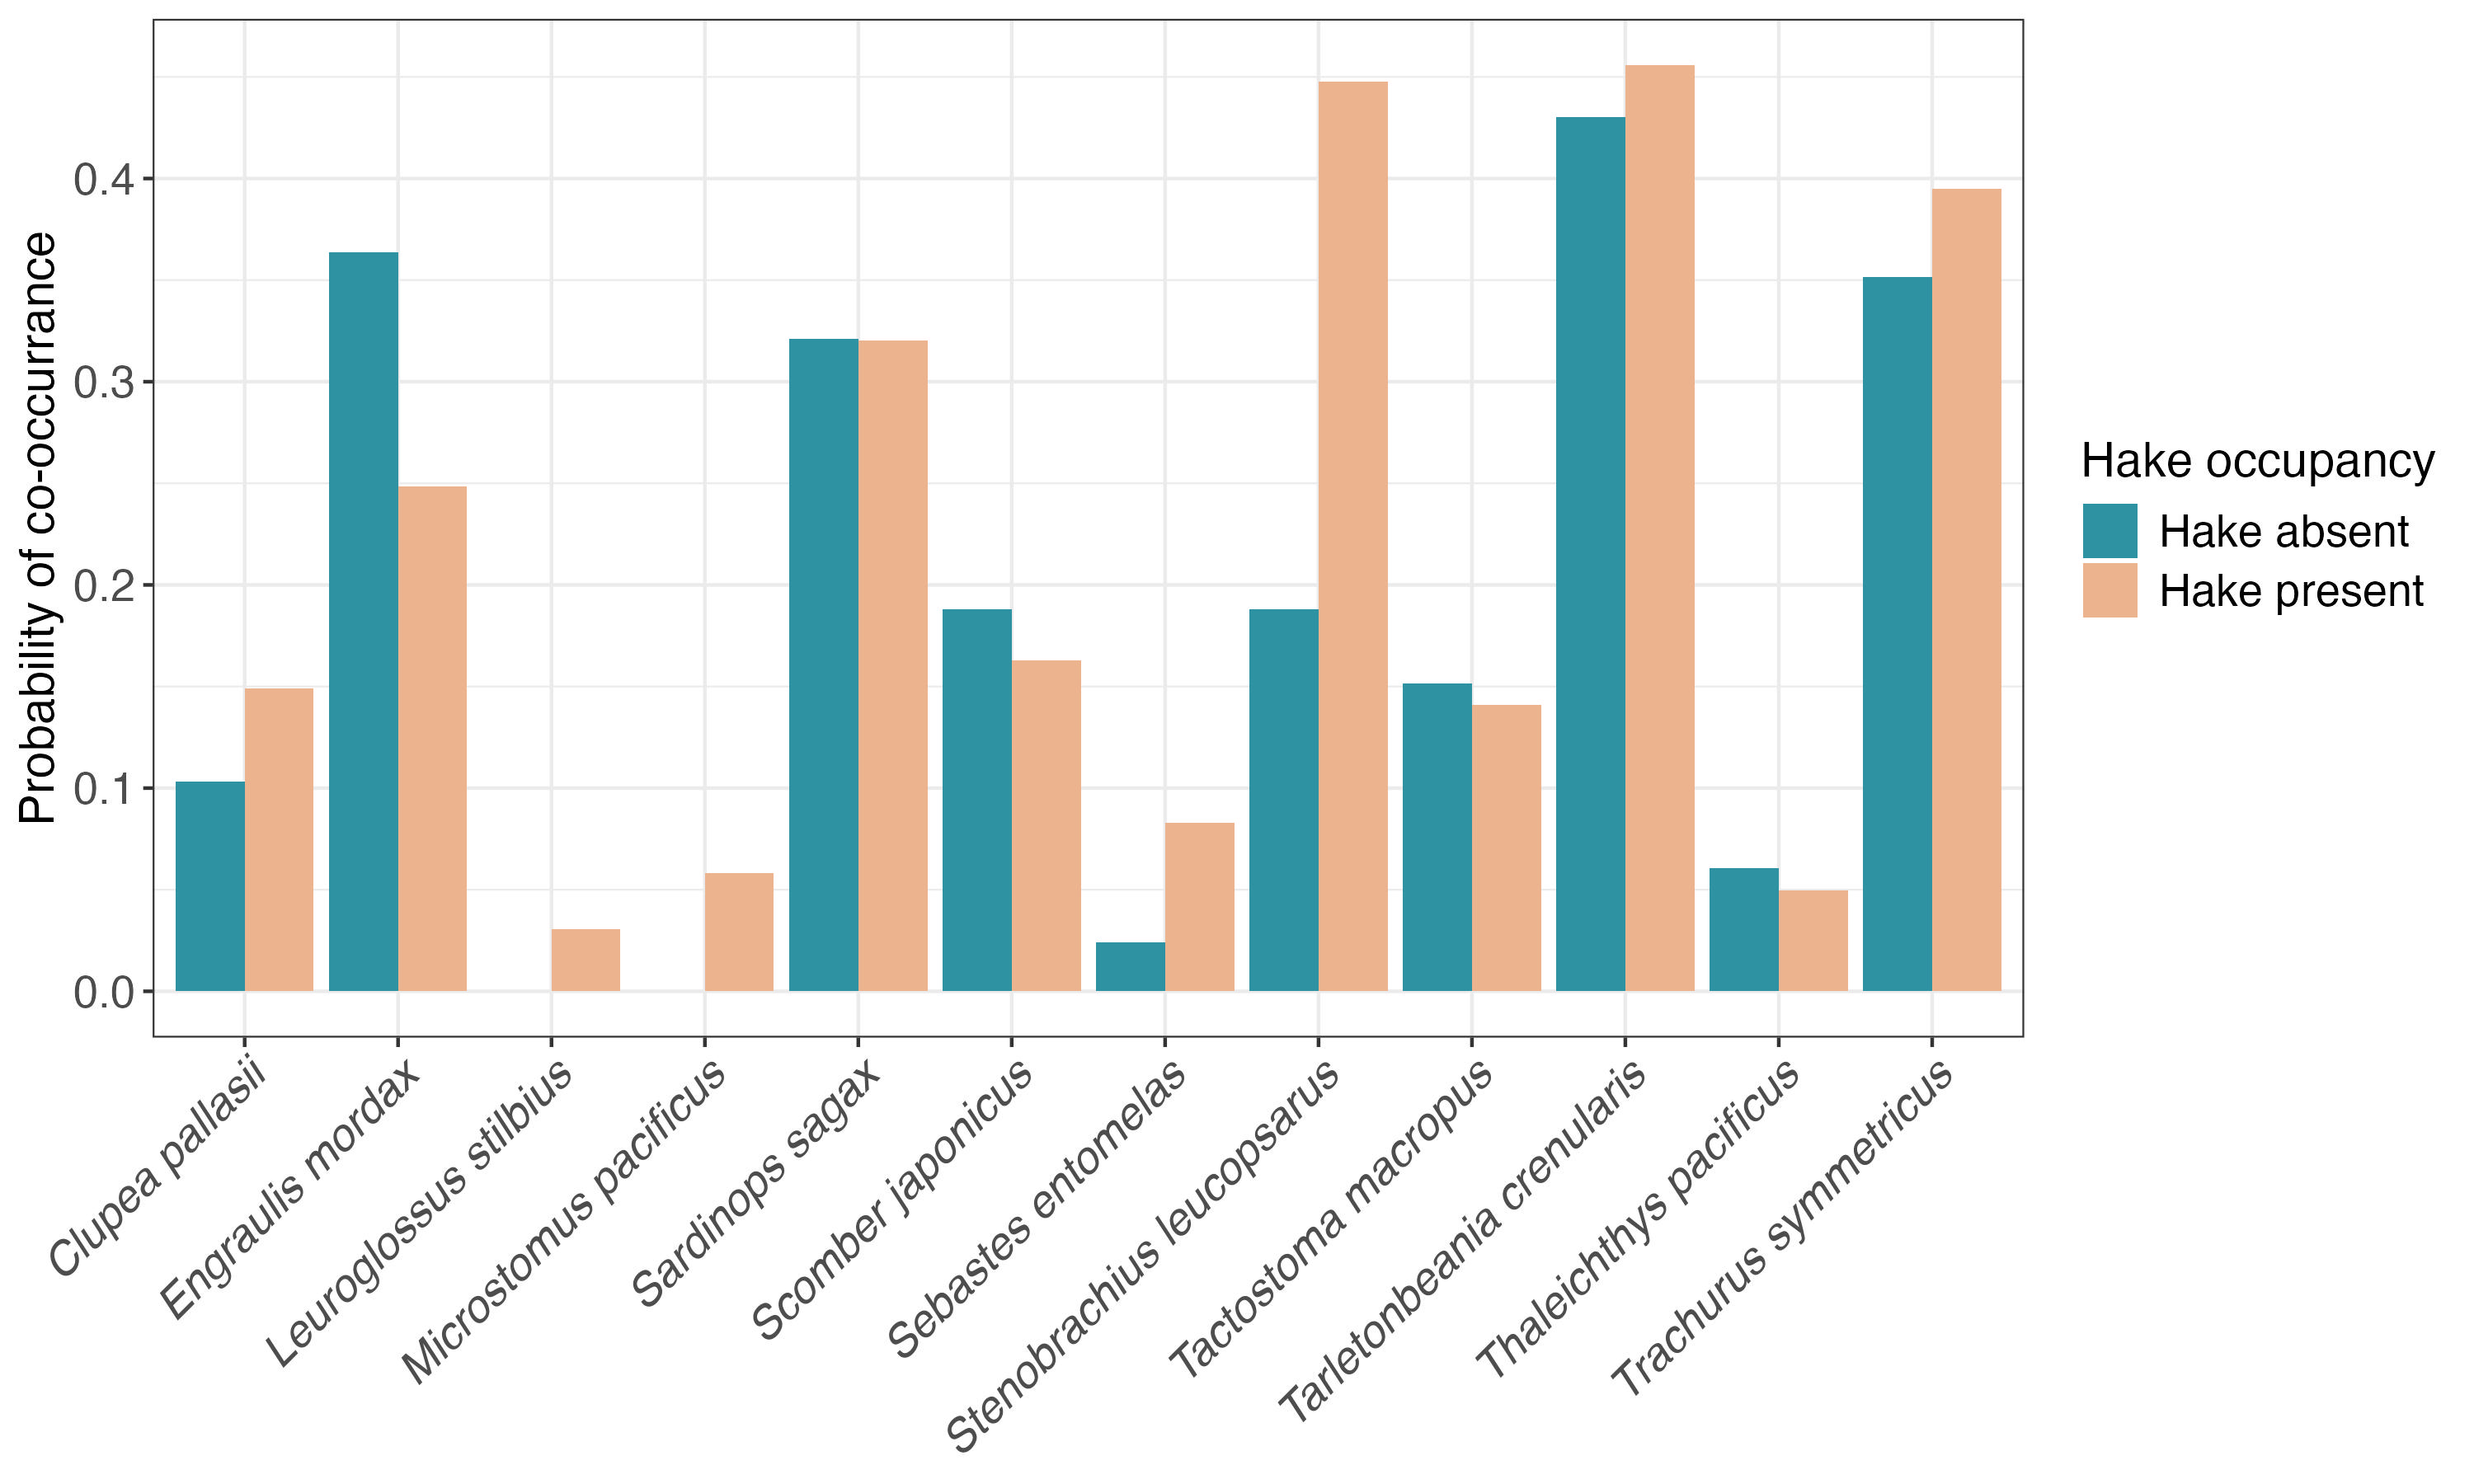
\includegraphics[width=0.99\textwidth]{plots/8_Supplementary_Figure_4.jpg}
\caption{Probability of species co-occurrence with Pacific hake, where blue bars represent non-occurrence and orange bars indicate co-occurrence. \textit{Engraulis mordax} exhibits the most inverse habitat overlap with hake, while \textit{Stenobrachius leucopsarus} shows the highest habitat overlap.}
\end{figure}

%%% Each figure should be on its own page
\begin{figure}
\centering
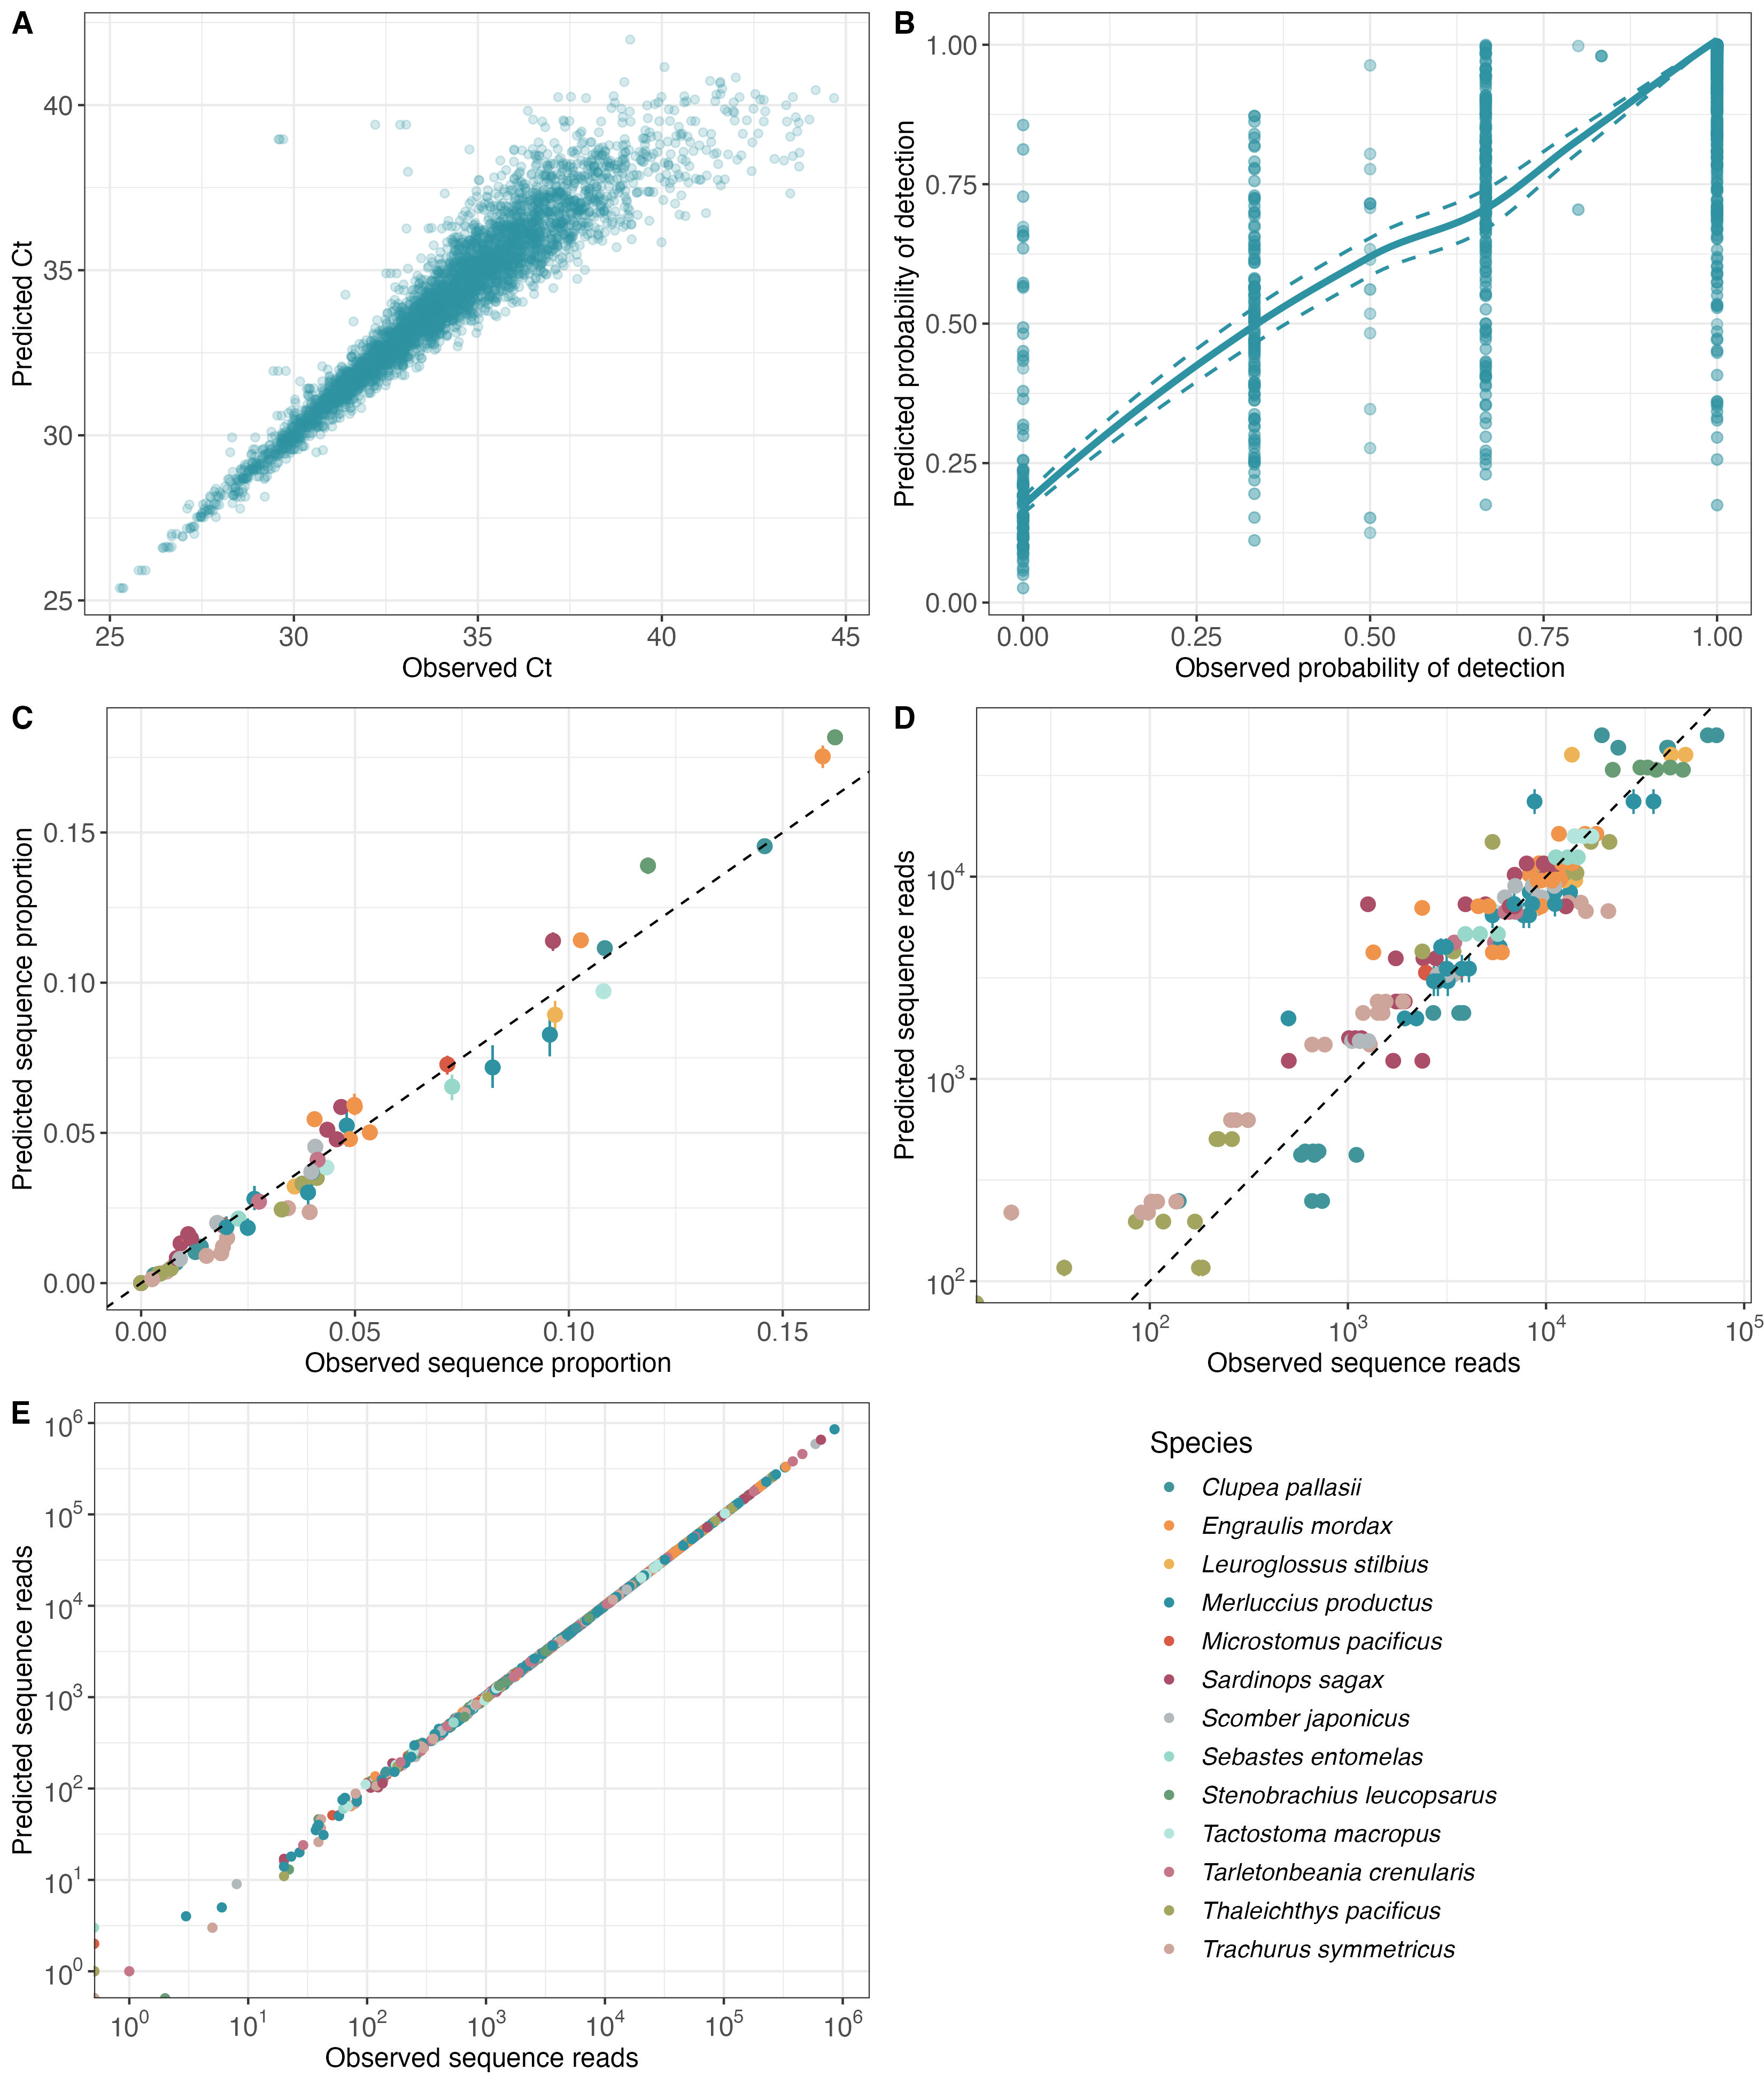
\includegraphics[width=0.98\textwidth]{plots/9_Supplementary_Figure_5.jpg}
\caption{Mean posterior predictions for three model compartments, qPCR continuous model (A), qPCR occupancy model (B), mock community model (C and D on species proportions and number of reads) and metabarcoding model (E)}
\end{figure}

%%% Each figure should be on its own page
\begin{figure}
\centering
\includegraphics[width=0.89\textwidth]{plots/10_Supplementary_Figure_6.jpg}
\caption{Estimated species eDNA concentration (copies/L) for all the species included in this study concentration across 0, 50, 150, 300, and 500m depth samples, without spatial smoothing.}
\end{figure}

\clearpage
\begin{table}\centering
\caption{Initial proportional abundances (measured by amplifying the 12S rRNA gene using MarVer1 primers \cite{valsecchi2020} and ddPCR QX200 Droplet Digital PCR system (Bio-Rad, Inc.)) of the selected species (n=12) across different mock communities (n=8). NA represent no DNA template included.}
    \begin{tabular}{lcccccccc}
        \toprule
        {Species} & \multicolumn{2}{c}{Mock1} & \multicolumn{2}{c}{Mock2} & \multicolumn{2}{c}{Mock3} & \multicolumn{2}{c}{Mock4} \\
        & Even & Skew & Even & Skew & Even & Skew & Even & Skew \\
        \midrule
        \textit{Clupea pallasii}           & 0.437 & 0.325  & 0.042  & 0.009     & -         & -          & 0.025      & 0.038 \\
        \textit{Engraulis mordax}          & 0.122 & 0.034  & 0.15 & 0.15       & 0.146      & 0.16       & 0.308      & 0.478 \\
        \textit{Leuroglossus stilbius}     & 0.108 & 0.29   & - & -         & -         & -         & -         & - \\    
        \textit{Merluccius productus}      & 0.079 & 0.144  & 0.12 & 0.06       & 0.117      & 0.075      & 0.247      & 0.287 \\
        \textit{Microstomus pacificus}     & -    & -     & 0.057  & 0.215     & -         & -         & -         & - \\    
        \textit{Sardinops sagax}           & 0.028 & 0.033  & 0.14 & 0.035      & 0.137      & 0.025      & 0.289      & 0.131 \\
        \textit{Scomber japonicus}         & -    & -     & 0.122  & 0.053      & 0.119      & 0.027     & -         & - \\    
        \textit{Sebastes entomelas}        & -    & -     & - & -          & 0.068      & 0.218     & -         & - \\    
        \textit{Stenobrachius leucopsarus} & -    & -     & - & -          & 0.356      & 0.487     & -         & - \\    
        \textit{Tactostoma macropus}       & -    & -     & 0.13 & 0.324     & -         & -         & -         & - \\    
        \textit{Tarletonbeania crenularis} & -    & -     & 0.083  & 0.124     & -         & -         & -         & - \\    
        \textit{Thaleichthys pacificus}    & 0.123 & 0.113  & 0.099  & 0.012     & -         & -          & 0.013      & 0.021 \\
        \textit{Trachurus symmetricus}     & 0.103 & 0.06   & 0.057  & 0.018      & 0.056      & 0.008      & 0.118      & 0.04 \\
        \bottomrule
    \end{tabular}
\end{table}
\clearpage

\begin{table}[h]
    \centering
    \begin{tabular}{lll}
         & \textbf{Description} & \textbf{Prior} \\
&Data & \\
\hline
$K$ & known DNA concentration from qPCR standards in copies/$\mu$L & - \\
$Z$ & qPCR amplification (yes=1; no=0) & - \\
$Y$ & qPCR cycle threshold (Ct) & - \\
$R$ & metabarcoding number of reads & - \\
$T$ & total number of reads for all S species & - \\
$N_{PCR}$ & number of metabarcoding PCR cycles & - \\
$L$ & known DNA concentration from mock commuinties in copies/$\mu$L & - \\
$V$ & volume filtered and aliquote dilution offset & -\\
$I$ & aliquote dilution factor & -\\

&&\\
&State processes&\\
\hline
$E$ & unknown DNA concentration in copies/$\mu$L & - \\
$D$ & unknown DNA concentration in copies/L & - \\
$F$ & smoothed DNA concentration in copies/L & - \\
&&\\

&Parameters&\\
\hline
$\psi$& mean hake eDNA concentration (copies/$\mu$L) & $\mathcal{N}(2,2)$\\
$\epsilon_{(x,y,d)}$& depth specific random effect & $\mathcal{N}(0,\tau)$\\
$\tau$& standard deviation of depth specific random effect & $\mathcal{N}(0,0.2)$\\
$\delta$& biological replicate random effect & $\mathcal{N}(0,\sigma_D)$\\
$\sigma_D$& standard deviation of biological replicate random effect  & $\mathcal{N}(0,3)$\\
$\phi$& intercept of the qPCR probability of detection relationship & $\mathcal{N}(3,1)$\\
$\beta0$& intercept of the linear relation between the mean Ct values&$\mathcal{N}(39,3)$\\
&and eDNA concentration (K and E) & \\
$\beta1$& slope of the linear relation between the mean Ct values and &$\mathcal{N}(-1.4,0.05)$\\
&eDNA concentration (K and E) & \\
$\gamma0$& intercept of the linear relation between the standard deviation&$\mathcal{N}(0,1)$\\
&of Ct values and eDNA concentration (K and E) & \\
$\gamma1$& intercept of the linear relation between the standard deviation &$\mathcal{N}(0,1)$\\
&of Ct values and eDNA concentration (K and E) & \\
$\alpha$& species amplification efficiency & fixed\\
$\zeta$& ethanol wash effect & fixed\\
&&\\
&Subscripts&\\
\hline
$s$& species ($H$ = Hake) & -\\
$x$& northing & -\\
$y$& easting & -\\
$d$& depth & -\\
$i$& biological replicate & -\\
$r$& technical replicate & -\\
$p$& qPCR plate & -\\
$m$& mock community sample & -\\
$j$& qPCR standard aliquote sample & -\\


    \end{tabular}
    \caption{Data, state processes, parameters, and subscripts employed in the joint Bayesian model and their prior distributions}
    \label{tab:filter_error}
\end{table}
\clearpage

\bibliography{Bib.bib}
\end{document}